\documentclass[dvipdfmx,a4j, titlepage]{jsarticle}
\usepackage{listings,jvlisting,array,tcolorbox,ascmac,siunitx,amsmath,amssymb,bm,here,float,comment,url}

\title{電気電子工学実験3 テーマS(a)\\ 簡単な4bit CPUの製作}
\author{三木 健太郎}
\date{2023年11月19日}
 
\begin{document}

\maketitle

\section{概要}
\subsection{製作物の概要}
本テーマ後半の自由設計では、簡単な4bit CPUの製作を行った。
このCPUはデータ転送命令や加算命令、データの入出力命令などを実行することができる。
これらの命令を組み合わせることで、LEDを予め決めた通りのパターンで光らせるプログラムや、
タイマー機能を持つプログラムなどを実行することができる。

\subsection{書籍「CPUの創りかた」について}
74シリーズの汎用論理ICを用い、データ転送・加算・データ入出力といった命令を実行できる4bit CPUを製作する方法を解説した書籍である。
LEDの点灯回路といった基本的な事項から、CPUの基本構成、実装方法といった応用的な事項まで、幅広い内容が平易に解説されている。
2003年に毎日コミュニケーションズ(現 マイナビ出版)から出版され、現在30刷以上重版されている。

\subsection{製作の動機}
計算機工学1や2で、フリップフロップなどのディジタル回路の基本的な構成要素やCPUの構造について学習した。
しかし、授業で知識を学んだだけでは、CPUの内部構造について、深い理解を得ることはできなかった。
そこで、本実験において簡単なCPUを実装することにより、CPUの内部構造を実感をもって理解したいと考えた。
簡単なCPUを実装するという内容の書籍は複数存在するが、回路自体の規模が大きく、授業時間内で実装を完遂するのが難しいものが多かった。
「CPUの創りかた」で解説されている「TD4」は、機能を絞っている分、回路の規模が小さく、授業時間内で実装を完遂することが可能であると考えた。

\subsection{制作方法}
基本的には、書籍「CPUの創りかた」に従って製作を行った。
具体的には、レジスタ、ALU、プログラムカウンタ、命令デコーダ、ROMの順に実装を行った。
書籍では74シリーズのICを用いながら実際に回路を組み立てるため、
解説内容がFPGAでの実装にそぐわない部分が一部あった。
そのような部分については、FPGAでの実装に適した内容に書き換えた。(詳細は後述する。)

\section{回路の説明}
\subsection{TD4の仕様}
TD4の命令長は8bitとなっており、オペコードが4bit、オペランドが4bitとなっている。
\footnote { 表現できるアドレスも4bitの範囲となるため、実行できるプログラムは最大で16ステップのものまでとなる。 }
演算用のレジスタはAレジスタとBレジスタの2つあり、いずれも4bitの値を記憶することができる。\\
TD4において実行できる命令の一覧を、 以下の表\ref{instruction_list}に示す。

\begin{table}[hbtp]
    \caption{TD4で実行可能な命令の一覧}
    \label{instruction_list}
    \centering
    \begin{tabular}{ccc}
        \hline
        命令                                  & オペコード & 概要                                                                       \\
        \hline \hline
        \verb|ADD A, Im|                & 0000       & Aレジスタに即値\verb|Im|を加算する                            \\
        \verb|ADD B, Im|                & 0101       & Bレジスタに即値\verb|Im|を加算する                            \\
        \verb|MOV A, Im|                & 0011       & Aレジスタに即値\verb|Im|を代入する                            \\
        \verb|MOV B, Im|                & 0111       & Bレジスタに即値\verb|Im|を代入する                            \\
        \verb|MOV A, B|                & 0001       & Bレジスタの値をAレジスタに代入する                                         \\
        \verb|MOV B, A|               & 0100       & Aレジスタの値をBレジスタに代入する                                         \\
        \verb|JMP Im|               & 1111       & 即値\verb|Im|で指定されたアドレスにジャンプする              \\
        \verb|JNC Im|               & 1110       & キャリーフラグが0のとき即値\verb|Im|のアドレスにジャンプする \\
        \verb|IN A|               & 0010       & 入力端子からデータを入力し、Aレジスタに代入する                            \\
        \verb|IN B|               & 0110       & 入力端子からデータを入力し、Bレジスタに代入する                            \\
        \verb|OUT B| \footnotemark & 1001       & Bレジスタの値を出力端子に出力する                                          \\
        \verb|OUT Im|               & 1011       & 即値\verb|Im|を出力端子に出力する                            \\
        \hline
    \end{tabular}
\end{table}
\footnotetext{なお、\verb|OUT A|命令は存在しない。}

\subsection{回路の全体像}
今回製作した回路の全体像を、以下の図\ref{circuit_diagram}に示す。

\begin{figure}[H]
    \begin{center}
        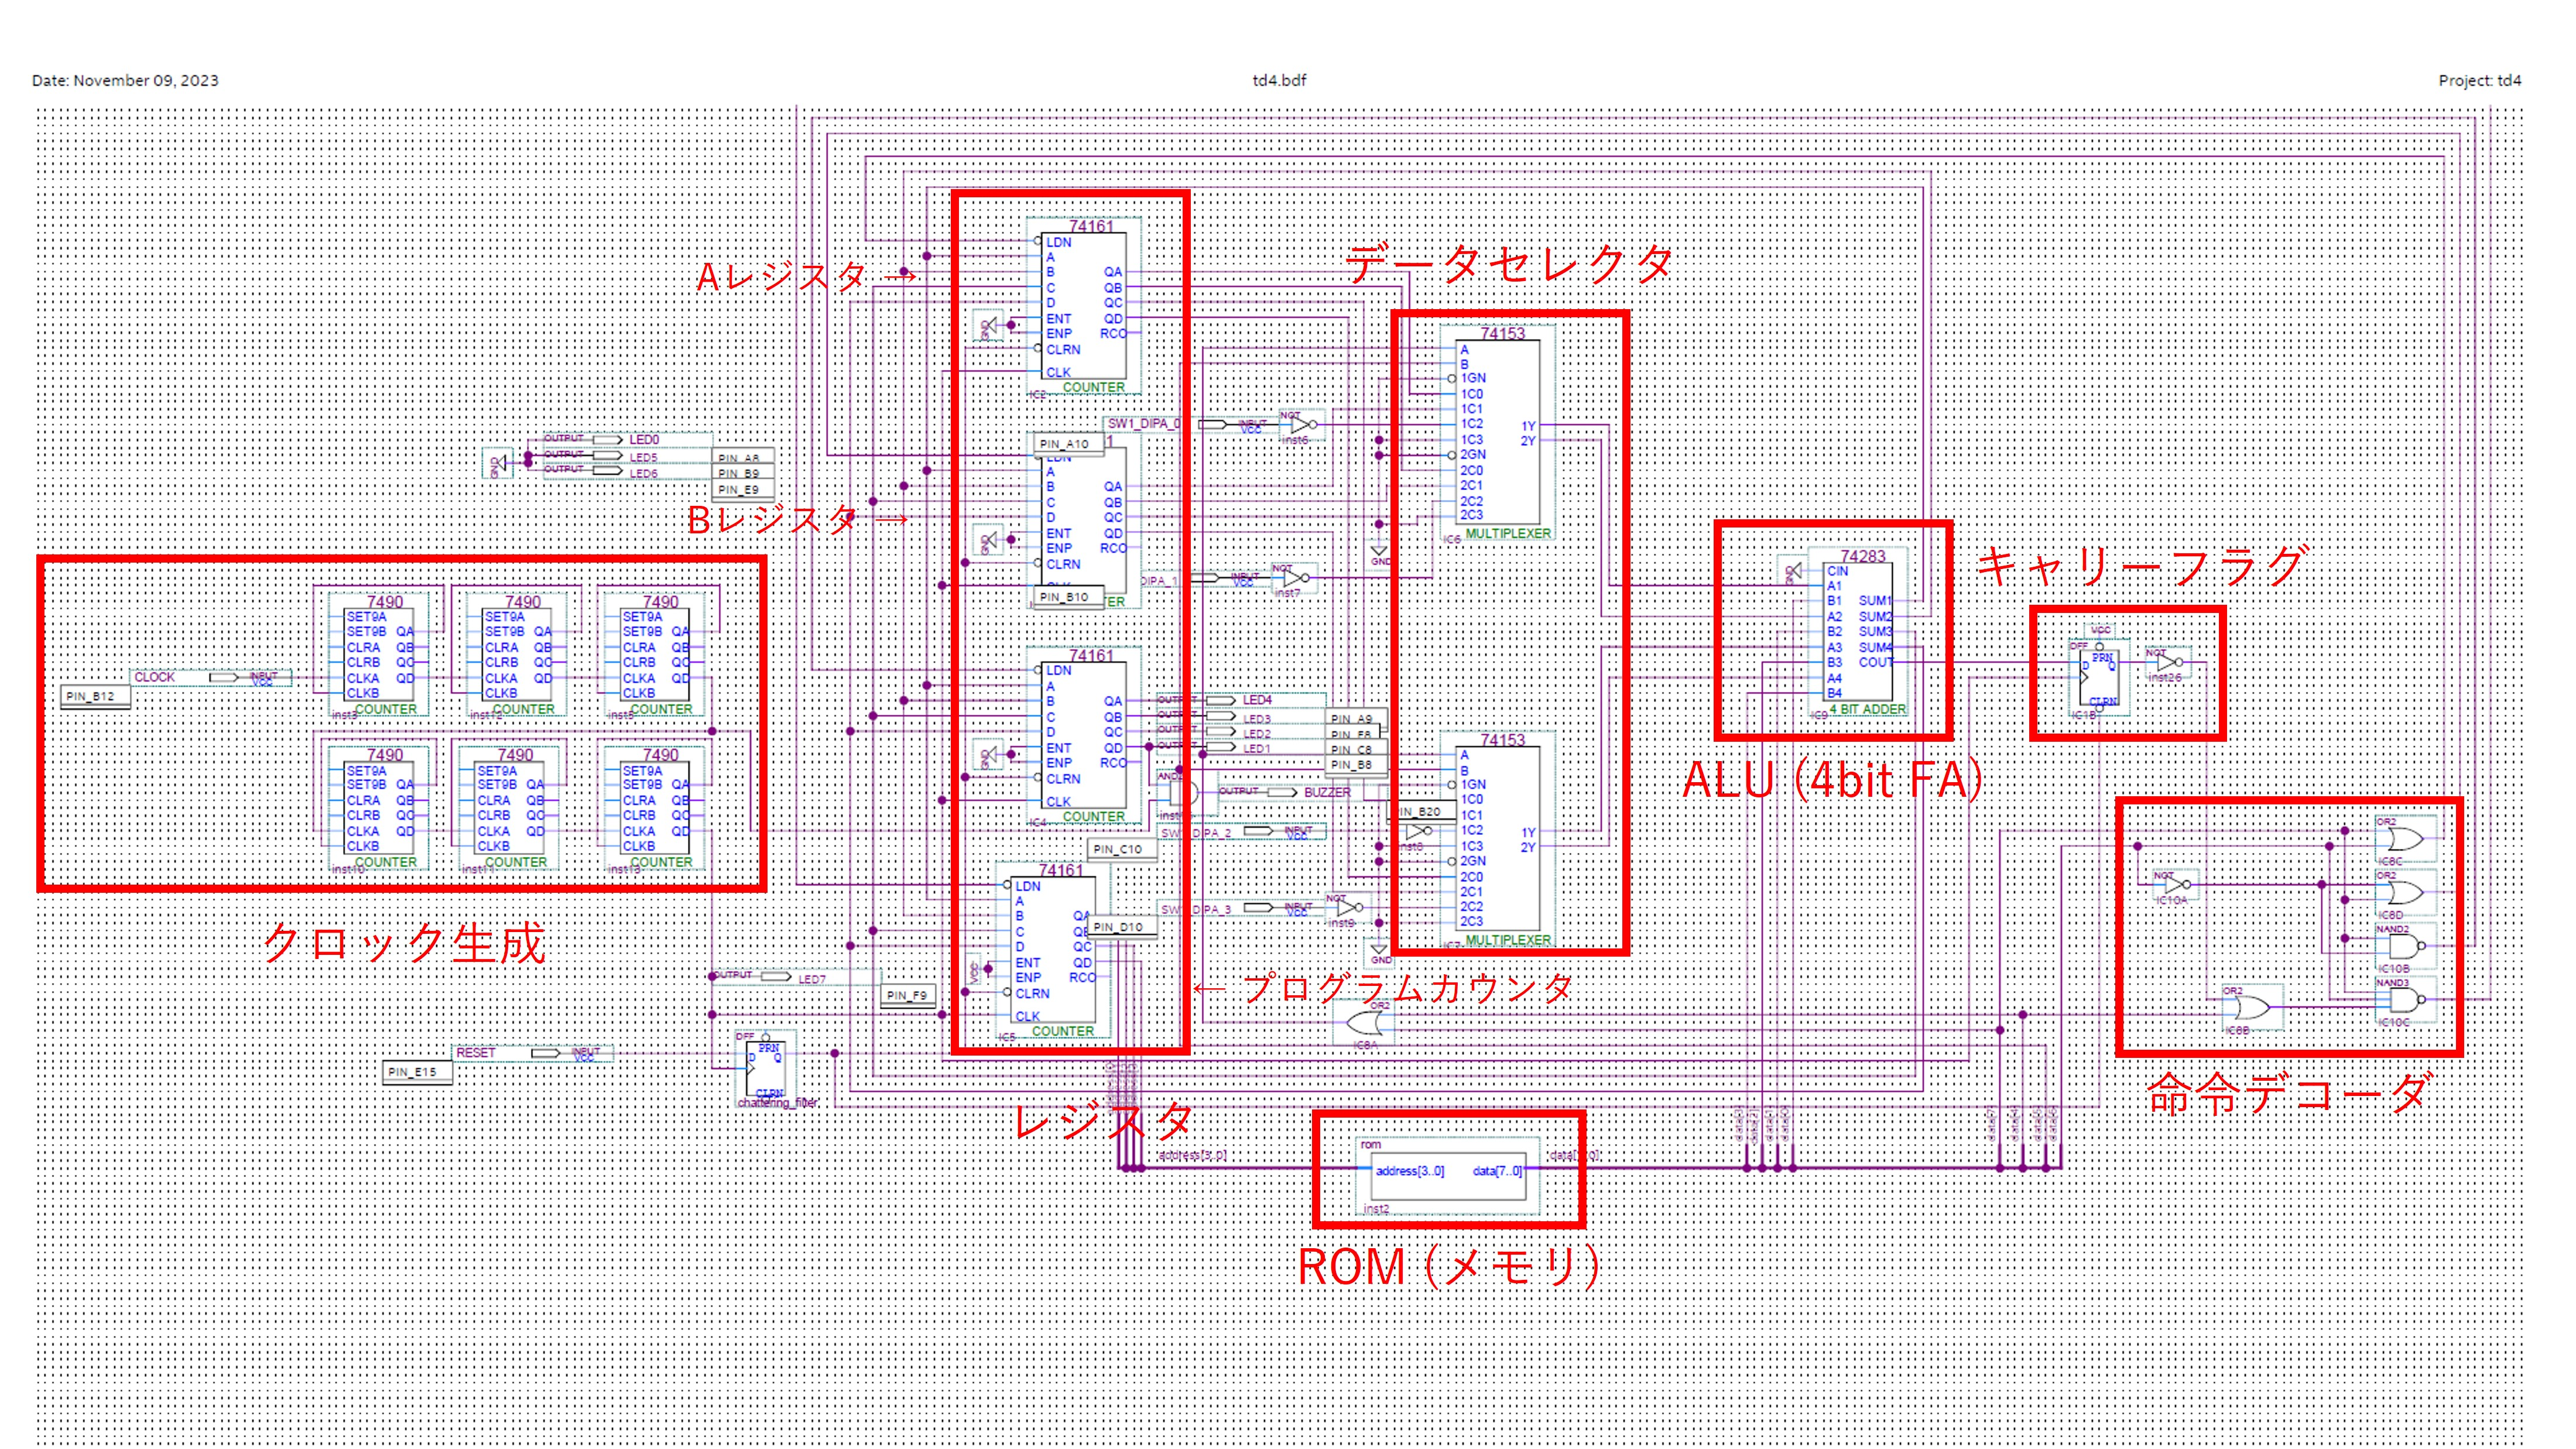
\includegraphics[width=165mm]{img/circuit_diagram.jpg}
    \end{center}
    \caption{製作した回路の全体像}
    \label{circuit_diagram}
\end{figure}

\end{document}
